\section{Data exploration}
\label{sec:data_exploration}

Fluorescent Neuronal Cells images are high-resolution RGB pictures of constant shape (1200 pixels height by 1600 pixels width) collected under fixed experimental conditions.
% In terms of data features, the most interesting aspects regard the color and luminance information, the counts distribution and the cells characteristics.
% In terms of data features, the most interesting aspects pertain the color and luminance information, the counts' distribution and characteristics of the cells.
The data can be explored at two complementary levels: pixel features and cell characteristics. 
On the one hand, interesting insights can be retrieved by looking at pixels' color and luminance information. Also, analogous analyses on the ground-truth masks reveal essential information about class-imbalance between signal and background.
On the other hand, examining object properties can highlight potential nuisances and suggest how to evaluate model performances.

The above data explorations are presented in the following sections of this chapter, and a summary table of the most important data features is reported in \cref{tab:data_features}.
\renewcommand{\cellalign}{cc}
\renewcommand{\theadalign}{cc}
\begin{table}[]
    \centering
    \resizebox{\textwidth}{!}{
    % \begin{tabular}{lrrrrrrrr}
    % \toprule
    % {} &          \thead{red\\intensity} &        \thead{green\\intensity} &         \thead{blue\\intensity} &  signal (\%) &  signal ratio &     area &  \thead{Feret\\diameter} &  \# cells \\
    % \midrule
    % mean &   7.32 &   2.83 &  0.20 &        0.50 &    366,681.94 & 1,212.18 &           55.71 &    27.05 \\
    % \thead{standard\\deviation}  &  16.81 &  13.30 &  1.43 &        0.61 &    755,628.42 &   995.40 &           26.12 &    21.75 \\
    % min  &   0 &   0 &  0 &        0 &         19.57 &   162 &           18.68 &     0 \\
    % 10\%  &   0 &   0 &  0 &        0 &         92.39 &   358 &           30.02 &     4 \\
    % 25\%  &   2 &   0 &  0 &        0.09 &        145.35 &   564 &           38.08 &     7 \\
    % 50\%  &   5 &   1 &  0 &        0.34 &        291.10 &   913 &           49.50 &    21 \\
    % 75\%  &   9 &   2 &  0 &        0.68 &      1,163.29 & 1,504 &           66.48 &    48 \\
    % 90\%  &  12 &   4 &  0 &        1.07 &  1,920,000 & 2,409 &           88.02 &    59 \\
    % max  & 252 & 251 & 87 &        4.86 &  1,920,000 & 8,092 &          215.10 &    68 \\
    % \bottomrule
    % \end{tabular}
    
    \begin{tabular}{lrrrrrrrr}
    \toprule
    {} &          \thead{red\\intensity} &        \thead{green\\intensity} &         \thead{blue\\intensity} &  signal (\%) &  signal ratio &     area &  \thead{Feret\\diameter} &  \# cells \\
    \midrule
    count & 1,919,905 & 1,919,910 & 1,919,955 &      283 &        283 & 2,137 &        2,137 & 2,193 \\
    mean  &         7.32 &         2.83 &         0.20 &        0.50 &    366,681.94 & 1,212.18 &           55.71 &    27.05 \\
    \thead{standard\\deviation}   &        16.81 &        13.30 &         1.43 &        0.61 &    755,628.42 &   995.40 &           26.12 &    21.75 \\
    min   &         0 &         0 &         0 &        0 &         19.57 &   162 &           18.68 &     0 \\
    10\%   &         0 &         0 &         0 &        0 &         92.39 &   358 &           30.02 &     4 \\
    25\%   &         2 &         0 &         0 &        0.09 &        145.35 &   564 &           38.08 &     7 \\
    50\%   &         5 &         1 &         0 &        0.34 &        291.10 &   913 &           49.50 &    21 \\
    75\%   &         9 &         2 &         0 &        0.68 &      1,163.29 & 1,504 &           66.48 &    48 \\
    90\%   &        12 &         4 &         0 &        1.07 &  1,920,000 & 2,409 &           88.02 &    59 \\
    max   &       252 &       251 &        87 &        4.86 &  1,920,000 & 8,092 &          215.10 &    68 \\
    \bottomrule
    \end{tabular}
    }
    \caption{\textbf{Distributions summary.} 
    Summary of the distributions illustrated in \cref{sec:data_exploration}. For each distribution we report the mean and standard deviation; minimum, maximum and 10\textit{-th}, 25\textit{-th}, 50\textit{-th}, 75\textit{-th} and 90\textit{-th} percentiles; the count of objects from which such measures are computed, i.e. pixels, images and cells.
    Notice that \textit{\# cells} count is obtained from the 2137 cells plus the 56 empty images.
    % Notice that commas are used as thousands separator
    }
    \label{tab:data_features}
\end{table}

\subsection{Salient features}
\label{sec:data_features}

% As far as the color, t
The picture appearance is dominated by two prevalent tints due to the intentional selection of a specific wavelength: a darker hue corresponding to areas whose light was filtered out and a yellow tone emitted by the fluorophore
(\cref{fig:dataset:empty,fig:artifacts}).
As a consequence, the only color channels to be populated are red and green, while blue is typically empty. 
An example of this effect is reported in \cref{fig:dataset:pixel_intensity}, where the average distribution of pixel intensity is illustrated (log scale).
\begin{figure}
    \centering
    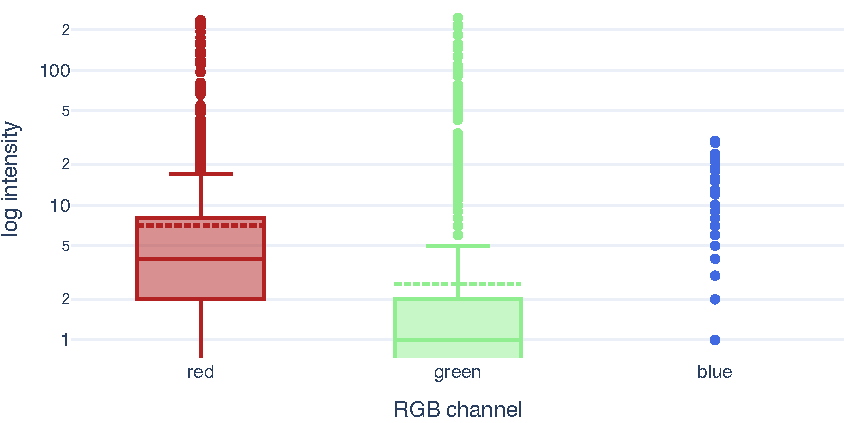
\includegraphics[width=\textwidth]{figures/120_dataset/features/pixel_intensity_distribution.pdf}
    \caption{\textbf{Pixel intensity distribution.} Violin plot of the average distribution of pixel intensities across the  RGB channels}
    \label{fig:dataset:pixel_intensity}
\end{figure}
In practice, the blues have an extremely narrow distribution squashed on zero, which makes it even difficult to visualize -- in fact only outliers are visible. 
The red and green channels are instead more populated. Their central tendency is still concentrated on low values due to the prevalence of background pixels, however we observe longer and thicker right tails, especially for the red channel (see \textit{red}, \textit{green} and \textit{blue} columns in \cref{tab:data_features} for a numeric summary).
Guided by this observation, one may argue that all this information is superfluous, so resorting to a grayscale transformation could be better since the images are ultimately shades of yellow.
A nice way to visually investigate such relationships is by exploring the colorspace representations of several images.
\Cref{fig:dataset:colorspace} reports the RGB and HSV encodings for two randomly sampled images.
Indeed, the RGB representations (\cref{fig:dataset:colorspace:rgb1,fig:dataset:colorspace:rgb2}) corroborate the previous intuition, as most pixels lay almost on a straight line in the red-green plane. 
This suggests that the two channels are highly correlated, so a one-dimensional subspace may be enough to represent most of the variability of the data.
In turn, this would bring two advantages: ease the learning process -- as neural networks typically suffer when inputs are correlated %\cite{} 
-- and make it more efficient -- as only one channel is considered instead of three.

However, the use-case at hand has no stringent requirements in terms of computing resources and runtime, so the 3-channels training is still feasible.
More importantly, the information thrown away when converting to grayscale, although tiny, may be crucial to discriminate background and signal. 
Hence, a 3D-encoding may still be worthed but the RGB colorspace may not be the optimal representation to learn this separation. A hint of that is demonstrated in \cref{fig:dataset:colorspace:hsv1,fig:dataset:colorspace:hsv2}, where the same images are depicted according to the HSV encoding. 
In this case, the separation between dark and colored tones appears more evident. 
Moreover, most of the pixels are concentrated in low hue values
and their distribution seems more spread across the saturation-value plane. 

All that being considered, we try to leverage the insights of both approaches. 
On one side, the RGB colorspace is taken as a starting point to retain all available information. On the other, the model first layer is designed to incorporate a colorspace transformation from RGB to a single channel.
% In this way, the intent is to avoid introducing any colorspace-related bias by letting the model learn the most convenient representation and, at the same time, benefit from the computational advantage due to a lower dimensionality.
% The intent is to avoid introducing any colorspace-related bias by letting the model learn the most convenient representation without ignoring the fact that a one-dimensional manifold is probably enough to express the variability of the data.
% The intent is to avoid introducing any colorspace-related bias by letting the model learn the most convenient representation.
% At the same time, by forcing the learned encoding to one dimension, we do not ignore the observation that a one-dimensional manifold is probably enough to express the data variability.
In this way, we avoid introducing any colorspace-related bias since the model learns the most convenient representation.
At the same time, we exploit the observation that a one-dimensional manifold is probably enough to express the data variability by forcing the learned encoding to one channel.
% \begin{figure}
%     \centering
%     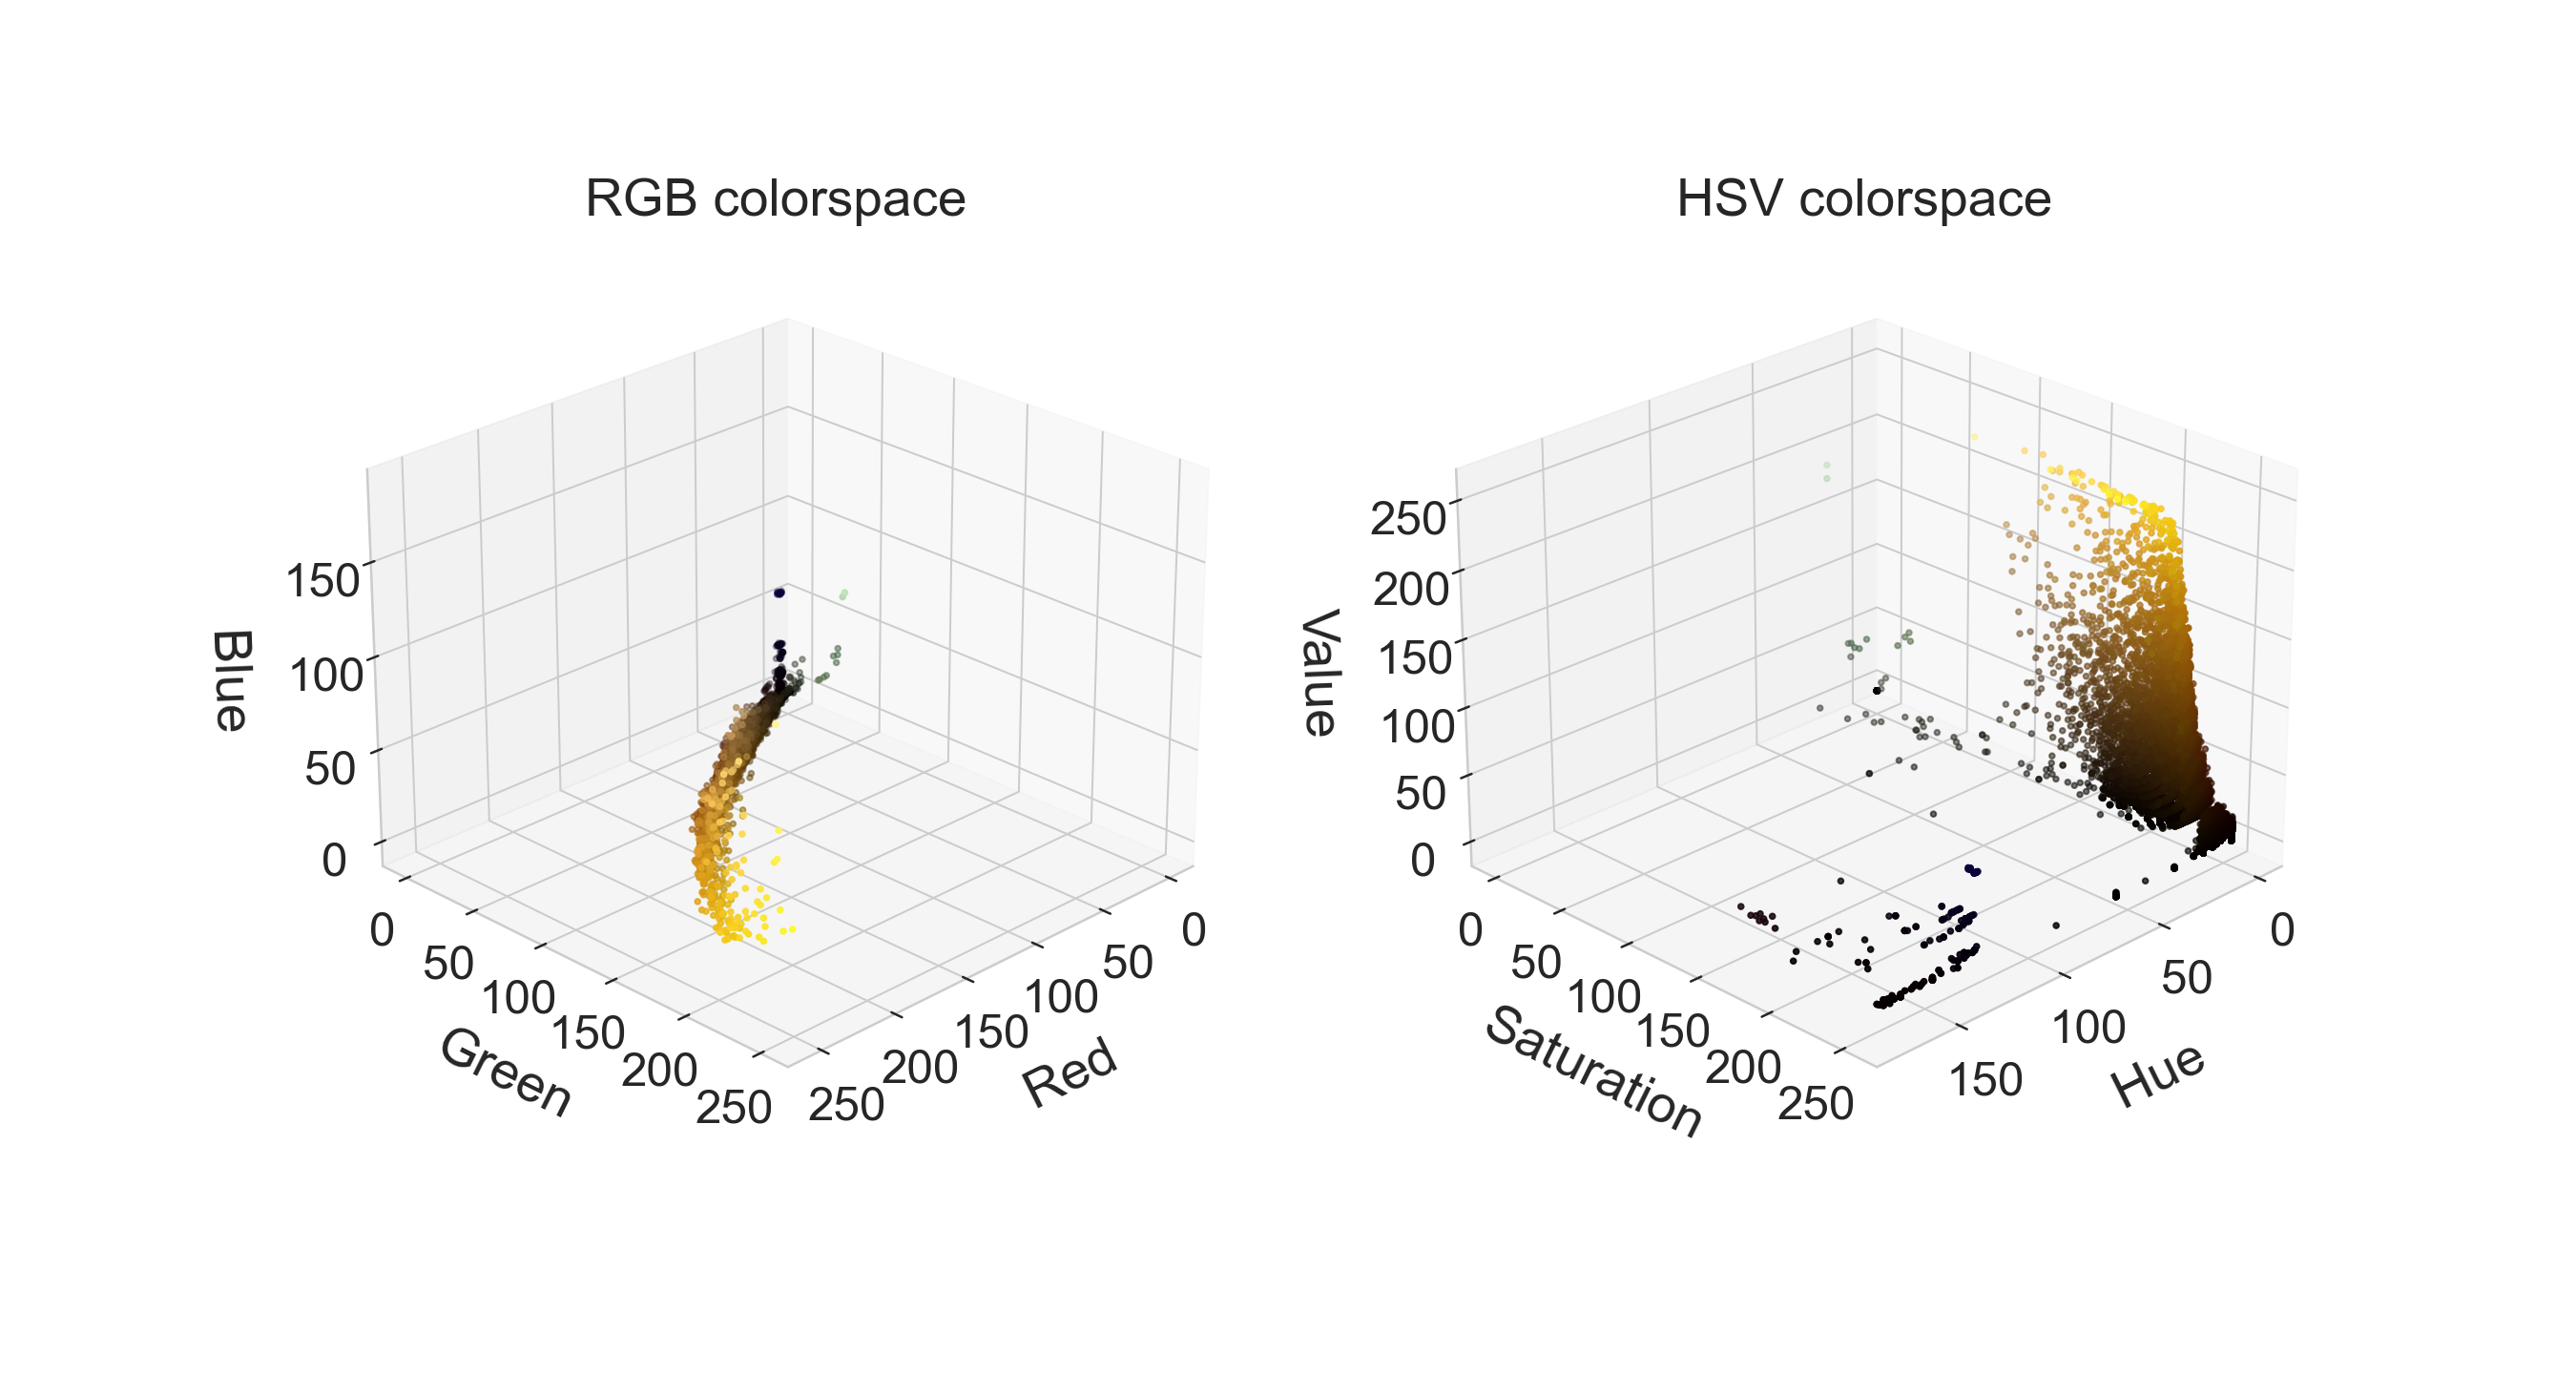
\includegraphics[width=1.1\textwidth]{figures/120_dataset/colorspace_Mar23bS1C2R3_VLPAGl_200x_y.png}
    
%     \centering
%     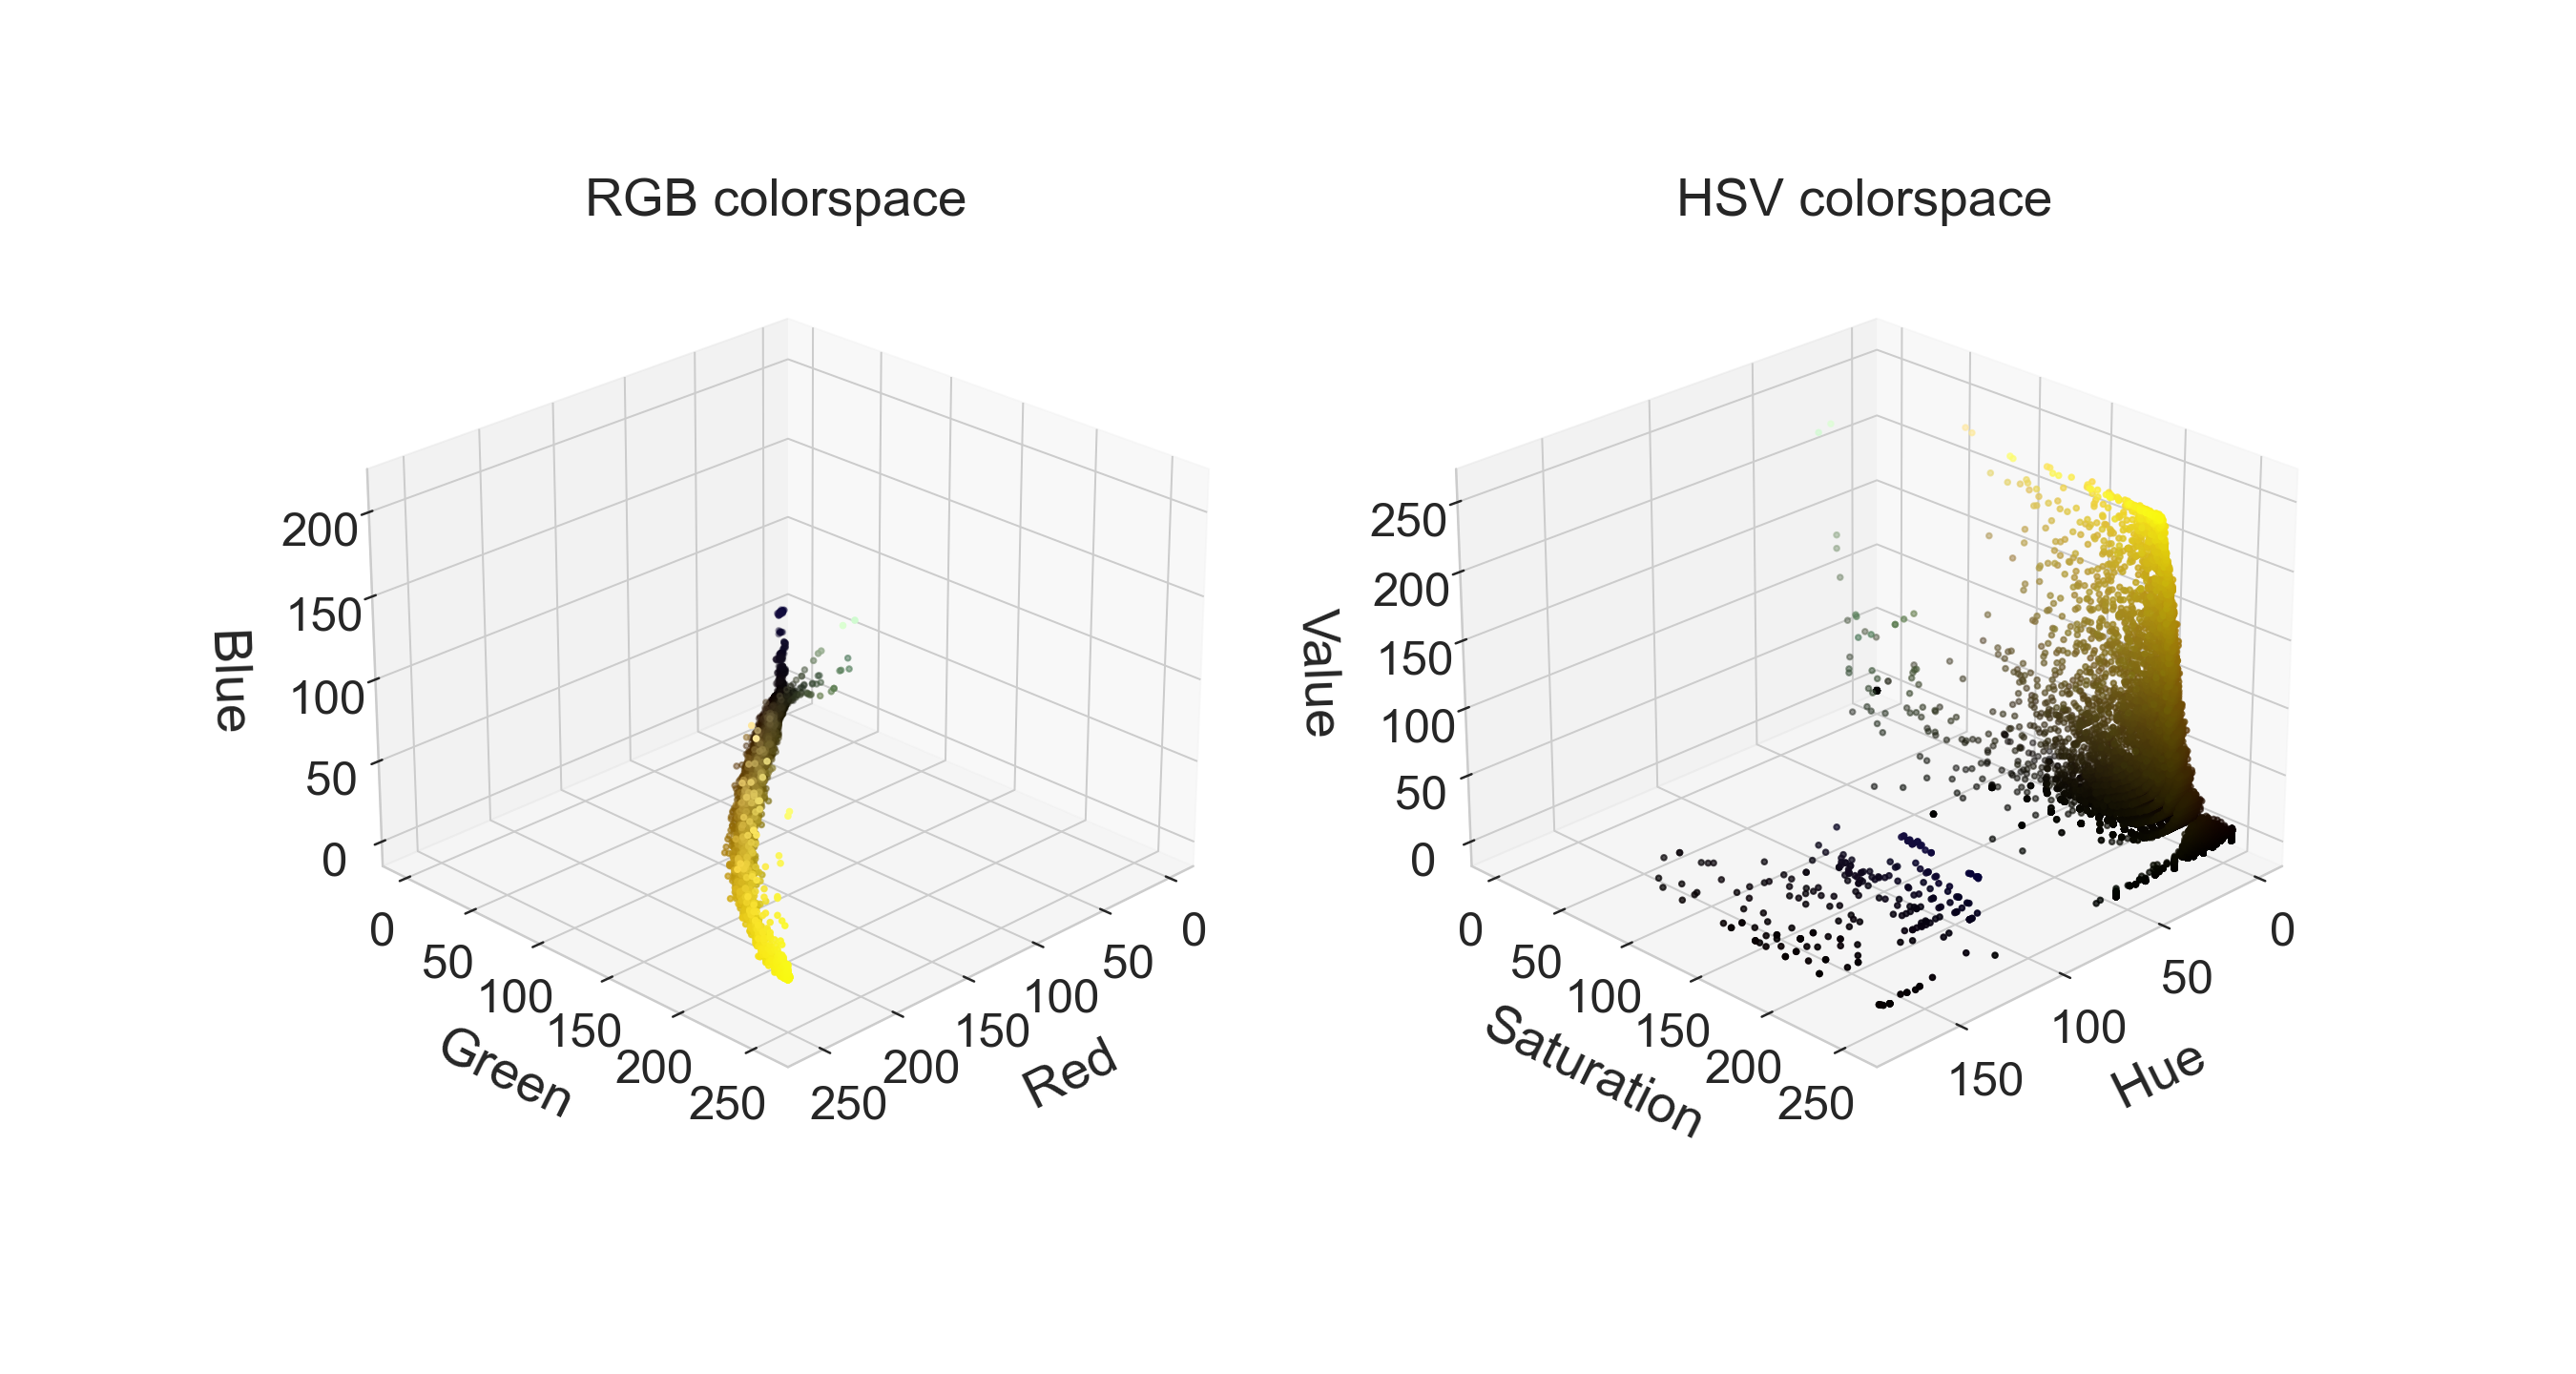
\includegraphics[width=1.1\textwidth]{figures/120_dataset/colorspace_Mar26bS2C1R2_DMl_200x_y.png}
%     \caption{Colorspace representation. The same image is represented as RGB (left) and HSV (right). Pixels are treated as 3D points with coordinates given by their encoding in the corresponding colorspace}
%     \label{fig:dataset:colorspace}
% \end{figure}
% \savegeometry{origigeom}
% \clearpage
% \newgeometry{lmargin=0.5cm}
\begin{figure}

    \centering
    Mar19bS1C4R3\_LHl\_200x\_y.png
    % \vspace{-3cm}
    \makebox[\textwidth][c]{\subfloat[RGB]{
    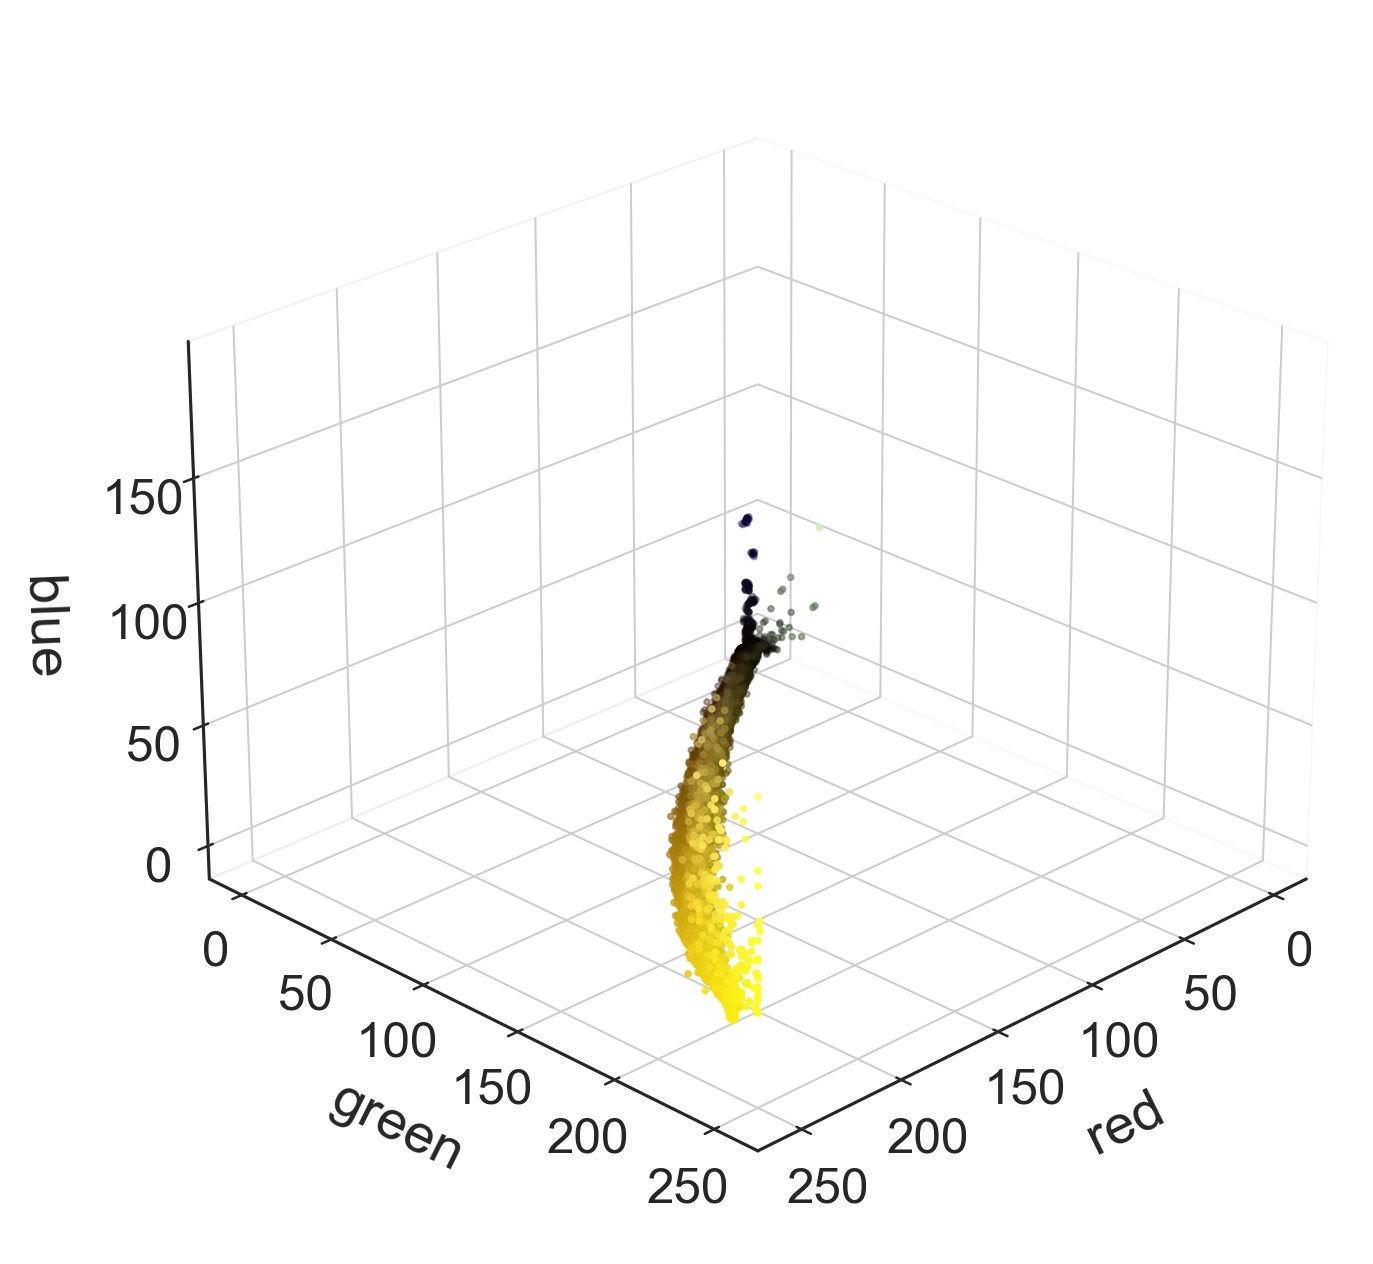
\includegraphics[width=0.55\textwidth]{figures/120_dataset/RGB_Mar19bS1C4R3_LHl_200x_y.png}\label{fig:dataset:colorspace:rgb1}
    }
    \subfloat[HSV]{
    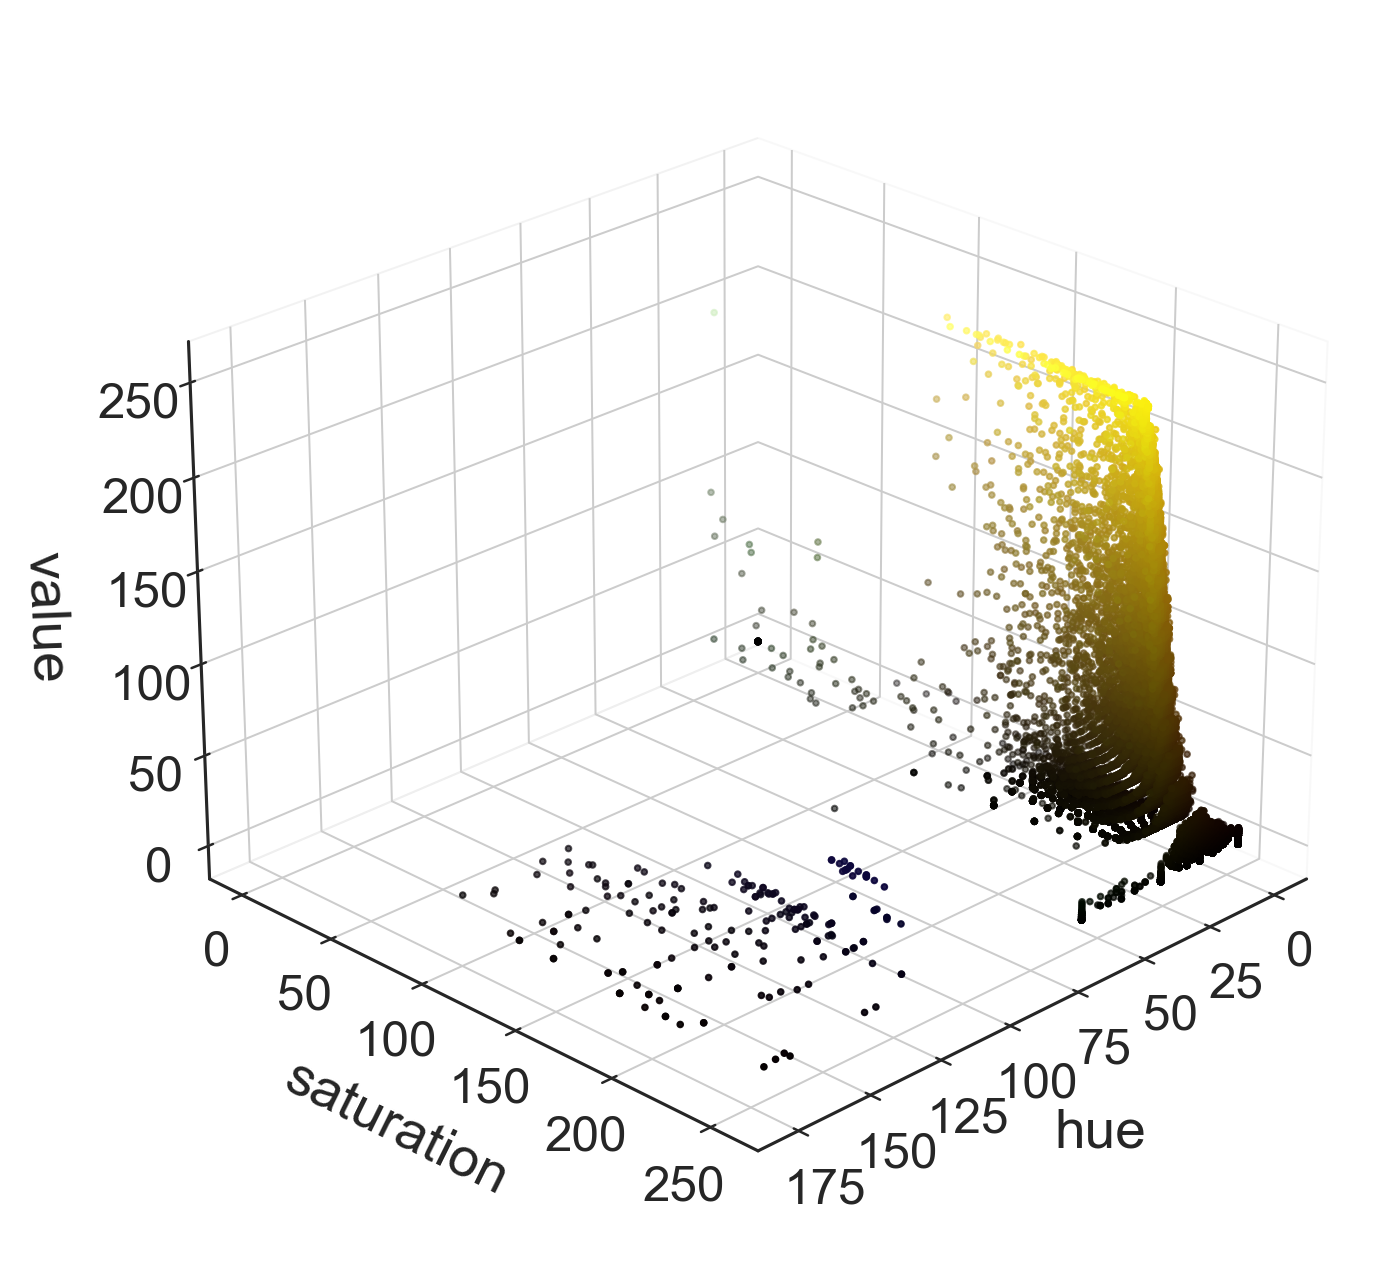
\includegraphics[width=0.55\textwidth]{figures/120_dataset/HSV_Mar19bS1C4R3_LHl_200x_y.png}\label{fig:dataset:colorspace:hsv1}
    }}
    
    \centering
    \vspace{1.5cm}
    Mar21bS1C1R3\_VLPAGl\_200x\_y.png   \makebox[\textwidth][c]{ \subfloat[RGB]{
    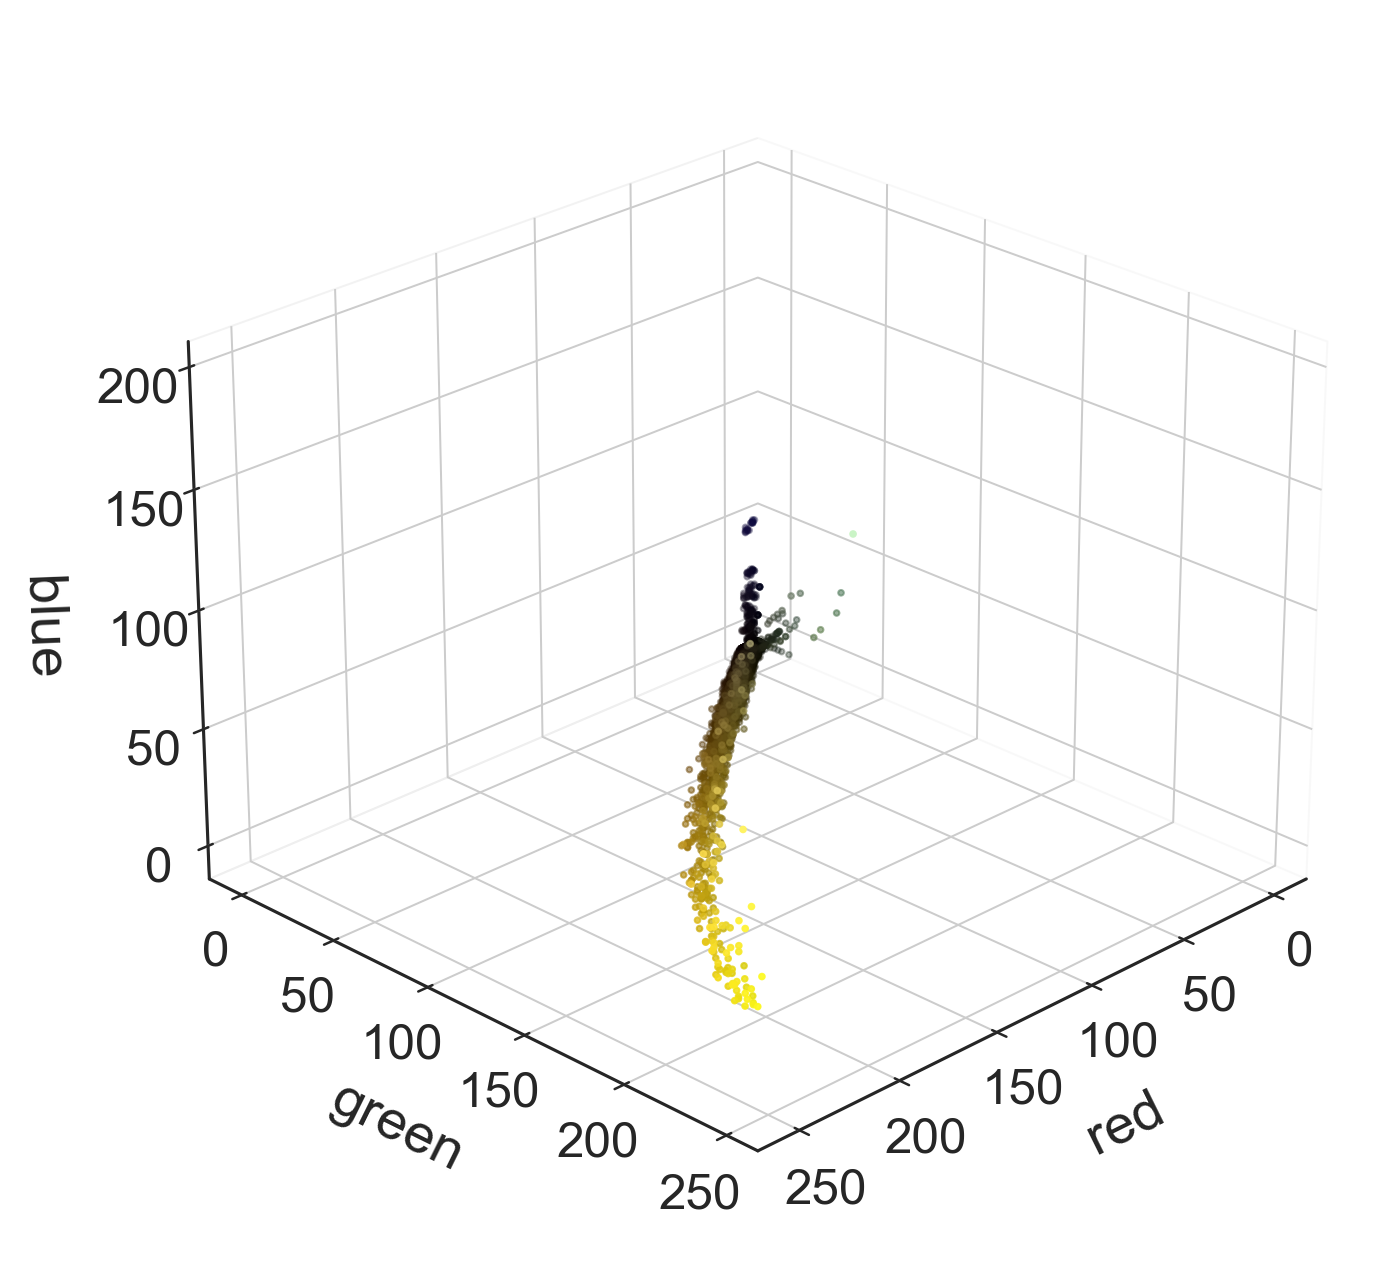
\includegraphics[width=0.55\textwidth]{figures/120_dataset/RGB_Mar21bS1C1R3_VLPAGl_200x_y.png}\label{fig:dataset:colorspace:rgb2}
    }
    \subfloat[HSV]{
    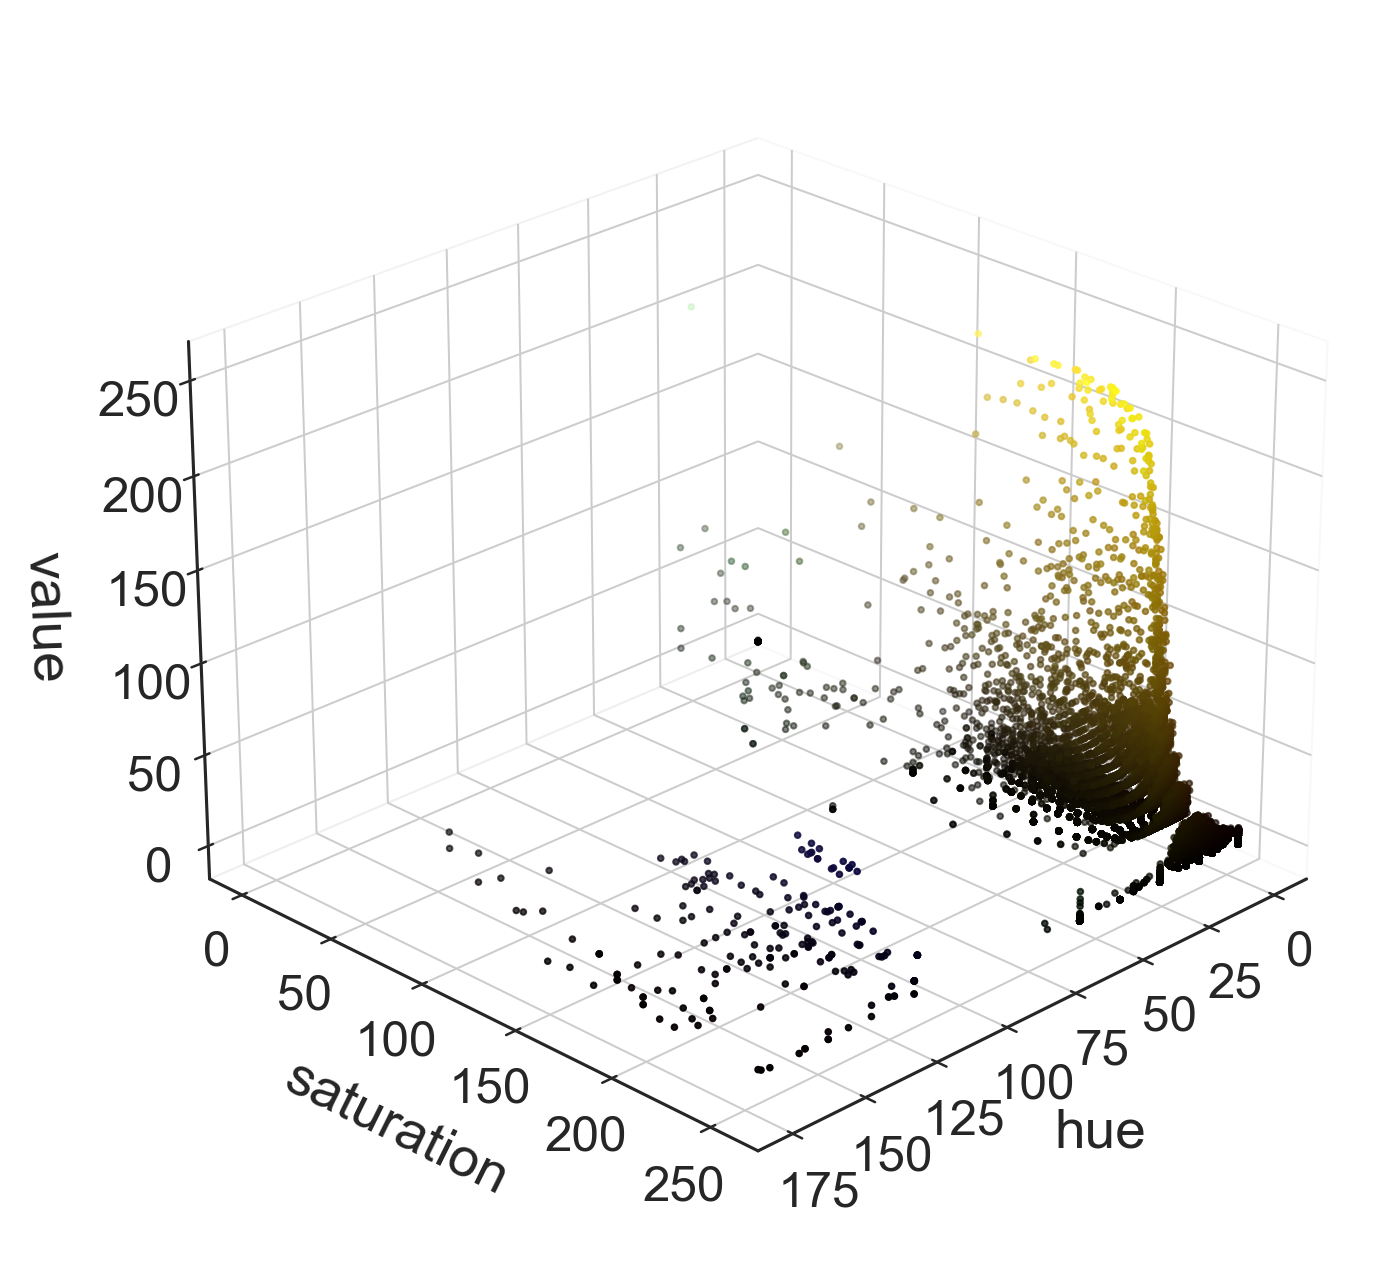
\includegraphics[width=0.55\textwidth]{figures/120_dataset/HSV_Mar21bS1C1R3_VLPAGl_200x_y.png}\label{fig:dataset:colorspace:hsv2}
    }}
    \caption{\textbf{Colorspace.} Two images represented as 3D points according to their RGB (left) and HSV (right) encodings. 
    Each point is colored as the corresponding pixel in the original image
    % The point color is the same as the pixel's color in the original image.
    }
    \label{fig:dataset:colorspace}
\end{figure}

% \clearpage
% \restoregeometry

\subsection{Class imbalance}
\label{sec:class_imbalance}
% \begin{figure}
%     \centering
%     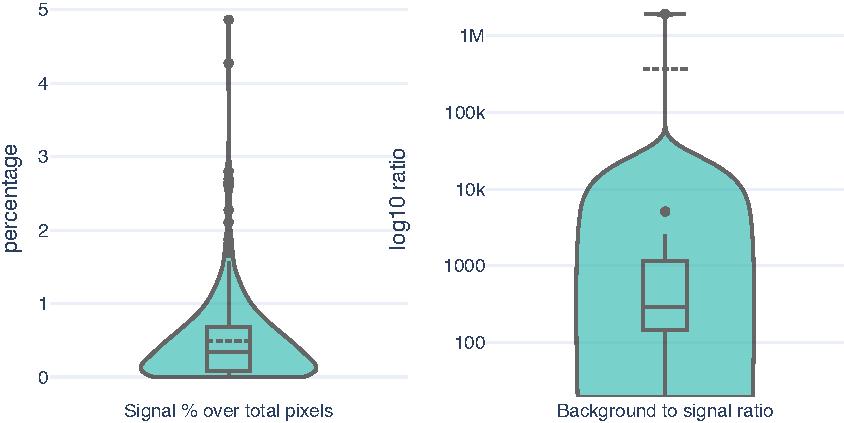
\includegraphics[width=\textwidth]{figures/120_dataset/features/class_imbalance.pdf}
%     \caption{\textbf{Class imbalance.} Violin plot and boxplot of signal percentage (left) and background to signal ration (right).}
%     \label{fig:dataset:class_imbalance}
% \end{figure}
\begin{figure}
    \centering
    \subfloat[Signal \% over total pixels]{
    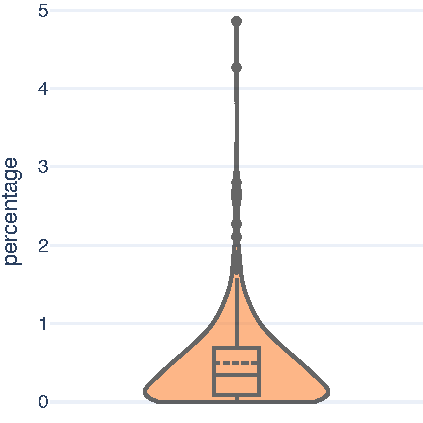
\includegraphics[width=0.5\textwidth]{figures/120_dataset/features/class_imbalance_percentage.pdf}\label{fig:dataset:class_imbalance:percentage}
    }
    \subfloat[Background to signal ratio]{
    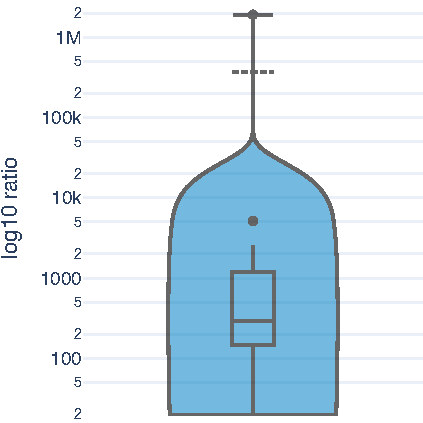
\includegraphics[width=0.5\textwidth]{figures/120_dataset/features/class_imbalance_ratio.pdf}\label{fig:dataset:class_imbalance:ratio}
    }
    \caption{\textbf{Class imbalance.} Violin plot and boxplot of signal percentage (left) and background to signal ration (right).}
    \label{fig:dataset:class_imbalance}
\end{figure}

Inspecting ground-truth masks at pixel level reveals important characteristics that affect the training process. 
By looking at the cardinality of pixels belonging to the background and the signal it is possible to notice how the two classes are extremely unbalanced (see \textit{signal (\%)}, and \textit{signal ratio} columns in \cref{tab:data_features} for a numeric summary).
\Cref{fig:dataset:class_imbalance:percentage} shows a violin plot of the percentage of signal pixel over the total image pixels across the 283 pictures.
The distribution is deeply skewed towards 0, with a median of 0.34\% and a 90\emph{-th} percentile of 1.07\%. 
Hence, almost 90\% of the images contain less than 1\% of pixels belonging to the signal%
% , causing an extreme unbalance between signal and background classes
.
Even more significantly, the right tail does not exceed 5\% of signal coverage, with a maximum of 4.86\%.

\Cref{fig:dataset:class_imbalance:ratio} illustrates the same concept but focuses on the relative proportion of background to signal. 
The distribution is left-skewed, with a lower half concentrated in the range (19, 291), i.e. background pixels are roughly from 20 to 300 times the signal pixels in 50\% of the images.
Remarkably, the disproportion grows even faster in the right tail, where the ratio explodes up to over 1000. 
Finally, notice that the bulk of outliers accumulates in the higher end of the domain. 
This is caused by the contribution of empty masks that cover more than 10\% of the total images.

These considerations expose the need for dedicated training strategies to face this strong class imbalance and correctly learn to classify image pixels.

\subsection{Objects features}
% \begin{figure}
%     \centering
%     \subfloat[Area]{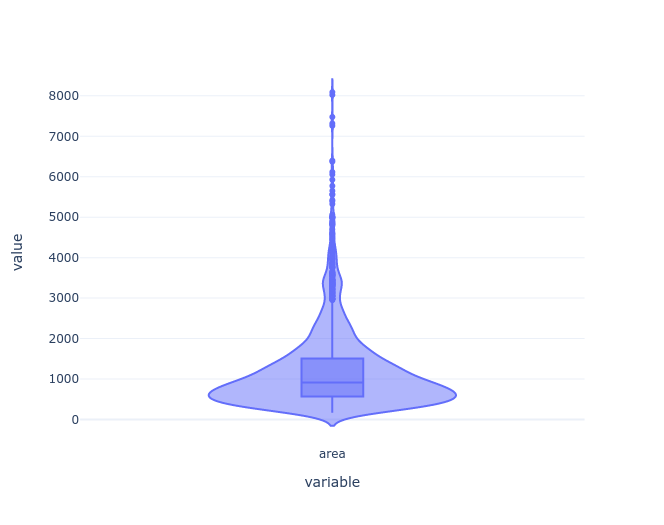
\includegraphics[width=0.5\textwidth]{figures/120_dataset/geometric_features area.png}
%     \label{fig:dataset:geom:area}
%     }
%     \subfloat[Feret diameter]{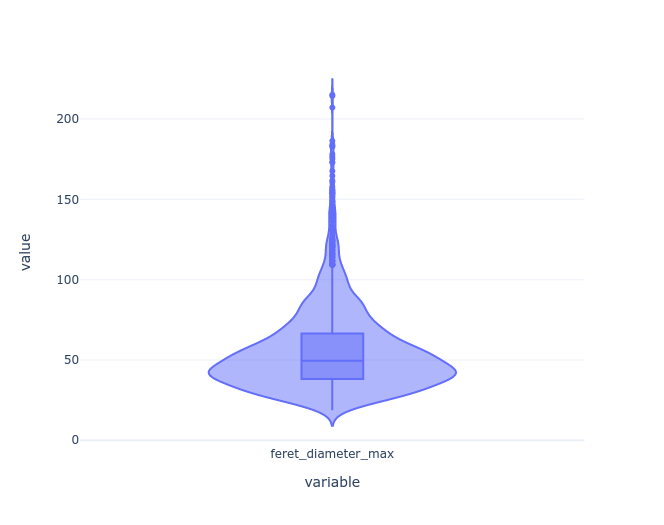
\includegraphics[width=0.5\textwidth]{figures/120_dataset/geometric_features feret.png}
%     \label{fig:dataset:geom:feret}
%     }
%     \caption{\textbf{Geometrical features.} Distributions of the area (left) and maximum Feret diameter (right) across all annotated cells.}
%     \label{fig:dataset:geom}
% \end{figure}
\begin{figure}
    \centering
    \subfloat[Area]{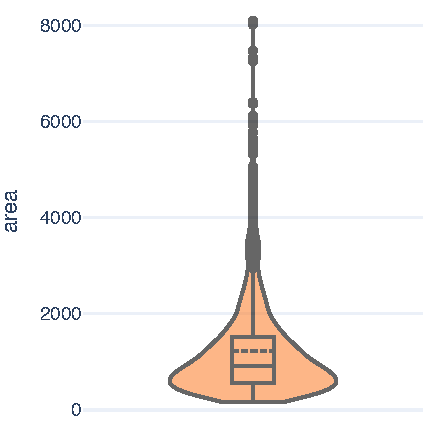
\includegraphics[width=0.5\textwidth]{figures/120_dataset/features/area.pdf}
    \label{fig:dataset:geom:area}
    }
    \subfloat[Feret diameter]{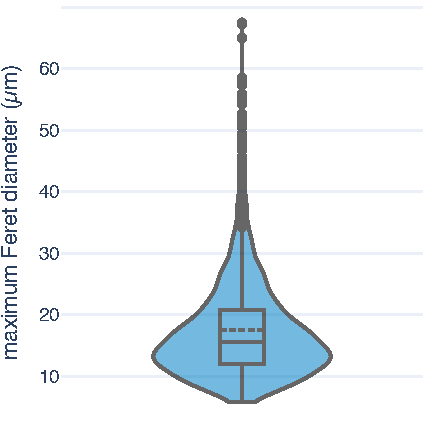
\includegraphics[width=0.5\textwidth]{figures/120_dataset/features/feret_diameter.pdf}\label{fig:dataset:geom:feret}
    }
    \caption{\textbf{Geometrical features.} Distributions of the area (left) and maximum Feret diameter (right) across all annotated cells.}
    \label{fig:dataset:geom}
\end{figure}
After the initial exploration of the data characteristics at the pixel level, additional investigations can be devoted to discovering meaningful insights about images' macroscopic content.
The Fluorescent Neuronal Cells pictures present a rich collection of 2137 neuronal cell instances of various shapes and sizes (see \textit{area}, and \textit{Feret diameter} columns in \cref{tab:data_features} for a numeric summary) that are unevenly distributed across the images.

\Cref{fig:dataset:geom} shows the distributions of the most interesting geometrical features of the annotated objects.
Regarding the area distribution (\cref{fig:dataset:geom:area}), the bulk of the distribution presents cells with a surface within 358 and 1504 pixels.
\Cref{fig:dataset:geom:feret} reports the maximum Feret diameter \cite{merkus2009particle} instead. This measure is computed as the longest distance (in pixels) between points of a convex cell countour\footnote{obtained using skimage package version `0.18.1'}.
The distribution extends from a minimum of 18 to a maximum of 215 pixels, with the central 50\% concentrated in the range [38, 66].
In both cases, the distribution is left-skewed, with a slight prevalence of values lower than the median.
In fact, 90\% of objects are small and medium cells with prevalently regular circular shapes, having an area within [162, 2409] pixels and a Feret diameter between 18 and 88.
The remaining 10\% of the distribution stretches up to a maximum of 8092 and 215, respectively.
This effect is due to the contribution of more oversized or prolonged objects that cause a long, heavy tail.

Finally, \ref{fig:dataset:counts_distrib} illustrates the distribution of the number of cells across the dataset (see \textit{\# cells} columns in \cref{tab:data_features} for a numeric summary).
In this case, the distribution presents multiple modes that can be summed up by the five major peaks, namely 6, 35, 38, 53 and 68
(\cref{fig:dataset:counts_hist}).
The empty spaces are a consequence of the fact that not all of the possible values were actually observed in the data.
Interestingly, a lower peak is observed at 0 because of the 56 images where no cells were annotated.

By looking at the estimated density in the violin plot (\cref{fig:dataset:counts_violin}), it appears that the distribution can be interpreted as a mixture of two components.
%In particular, one can distinguish two peaks by looking at the estimated density in \cref{fig:dataset:counts_violin}.
The first is centered around 6 and is made of the images with lower counts, i.e. the ones depicting brain areas where the fluorophore did not yield abundant emissions.
The second, instead, is a combination of the four higher peaks that represent active brain areas.
% \begin{figure}
%     \centering
%     \subfloat[Histogram]{
%     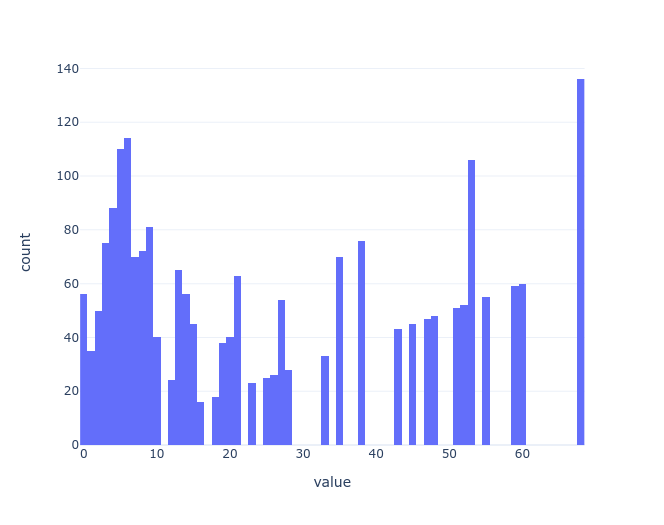
\includegraphics[width=0.5\textwidth]{figures/120_dataset/counts_histogram.png}
%     \label{fig:dataset:counts_hist}
%     }
%     \subfloat[Violin plot]{
%     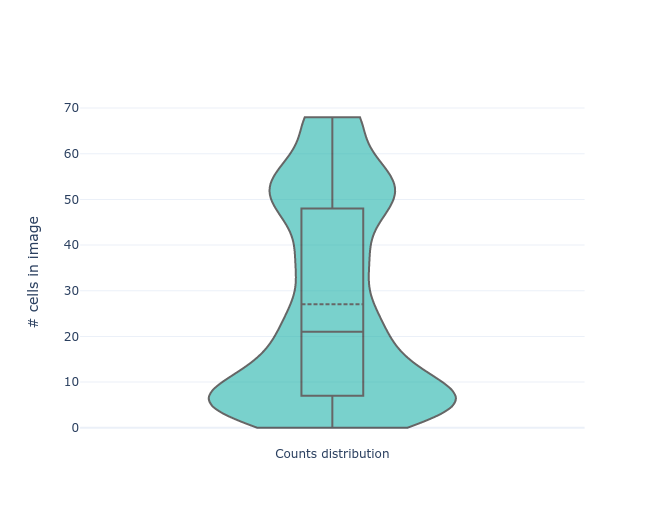
\includegraphics[width=0.5\textwidth]{figures/120_dataset/counts_violin.png}
%     \label{fig:dataset:counts_violin}
%     }
%     \caption{\textbf{Counts distribution.} Distributions of the number of annotated cells across all images in the dataset.}
%     \label{fig:dataset:counts_distrib}
% \end{figure}


\begin{figure}
    \centering
    \subfloat[Histogram]{
    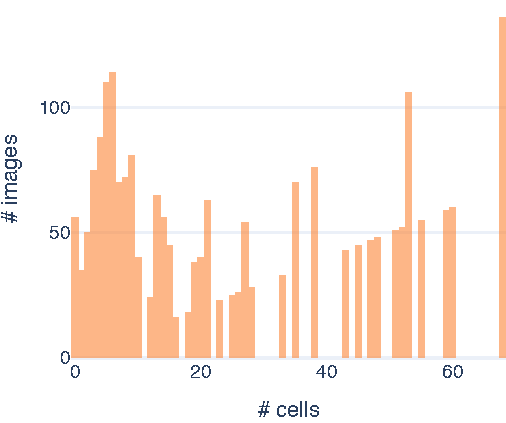
\includegraphics[width=0.6\textwidth]{figures/120_dataset/features/count_histogram.pdf}
    \label{fig:dataset:counts_hist}
    }
    \subfloat[Violin plot]{
    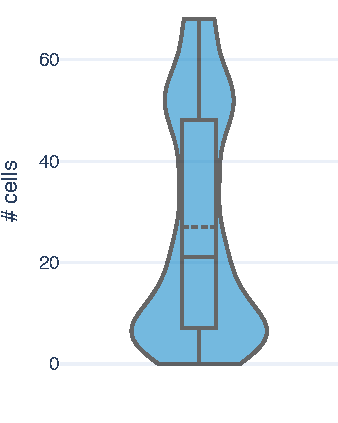
\includegraphics[width=0.4\textwidth]{figures/120_dataset/features/count_violin.pdf}
    \label{fig:dataset:counts_violin}
    }
    \caption{\textbf{Counts distribution.} Distributions of the number of annotated cells across all images in the dataset.}
    \label{fig:dataset:counts_distrib}
\end{figure}